\newpage
\section{Anhang}

\begin{figure}[h]
  \centering
  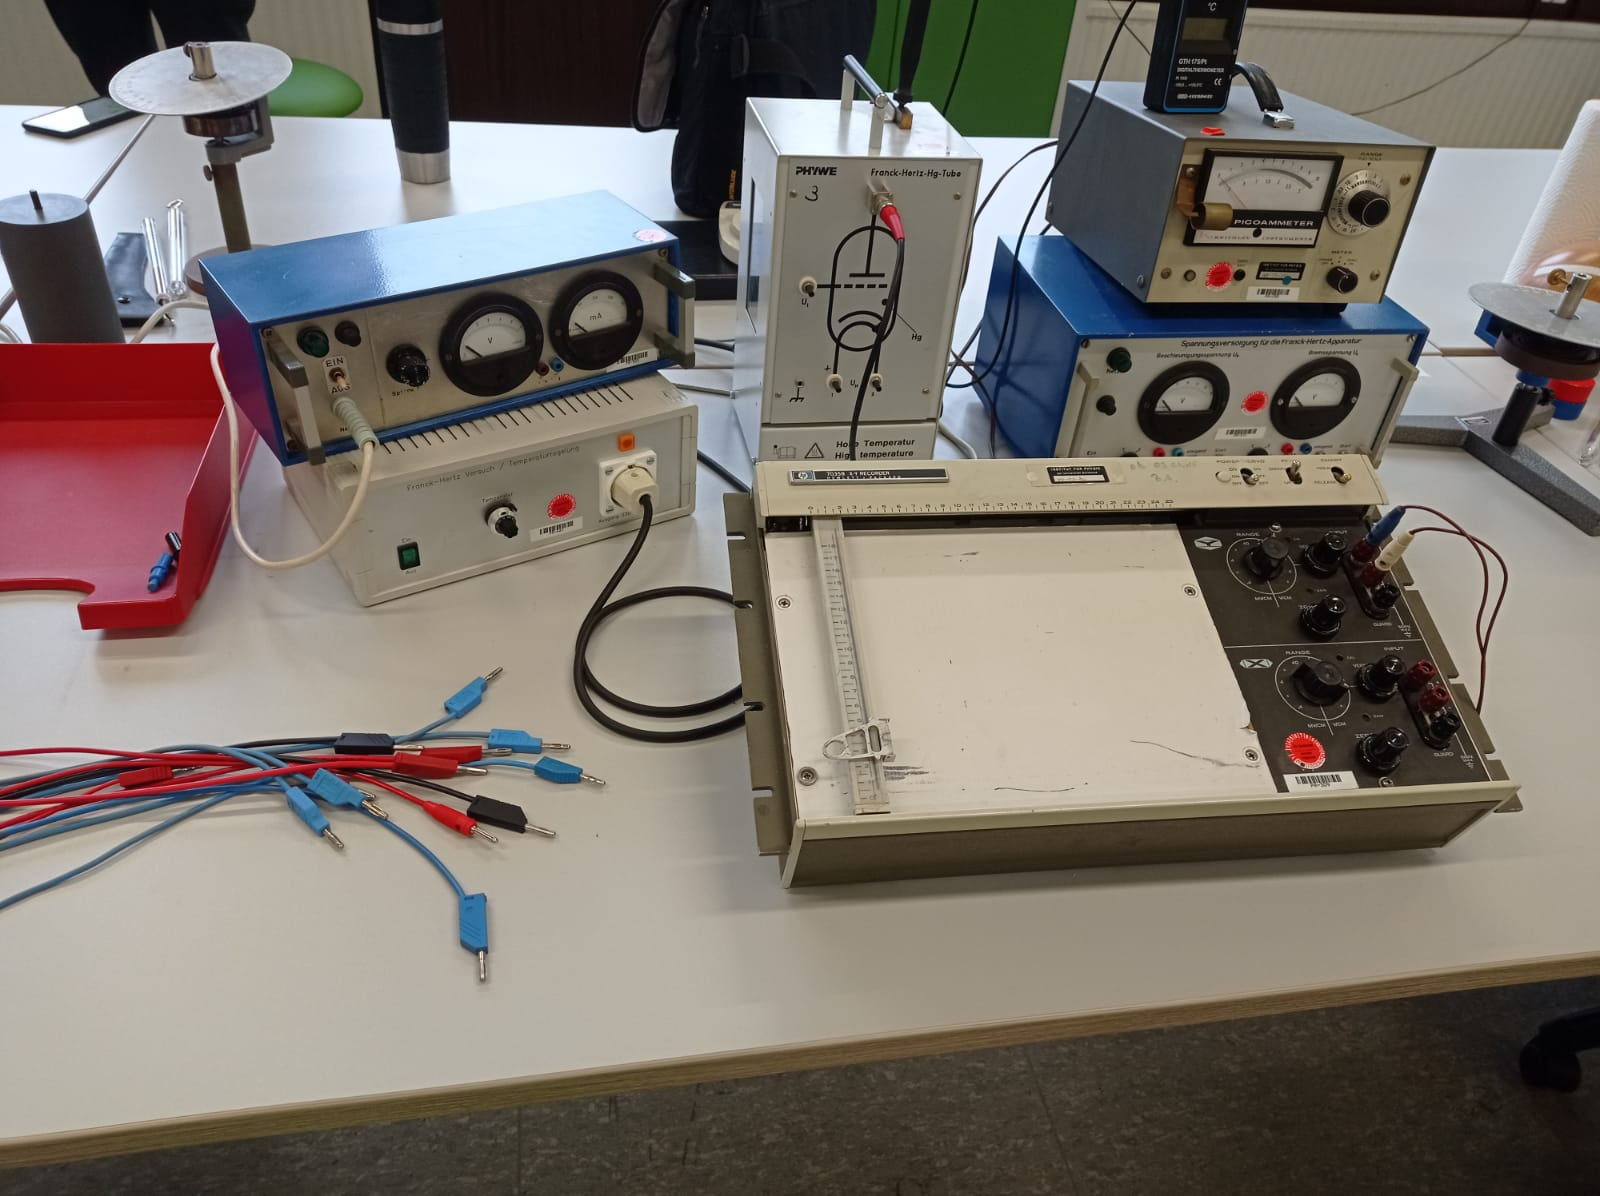
\includegraphics[width=0.7\textwidth]{latex/images/aufbau.jpeg}
  \caption{Die vom x-y-Schreiber erstellten differentiellen Energieverteilungen.}
  \label{img:mess1}
\end{figure}

\begin{figure}[h]
  \centering
  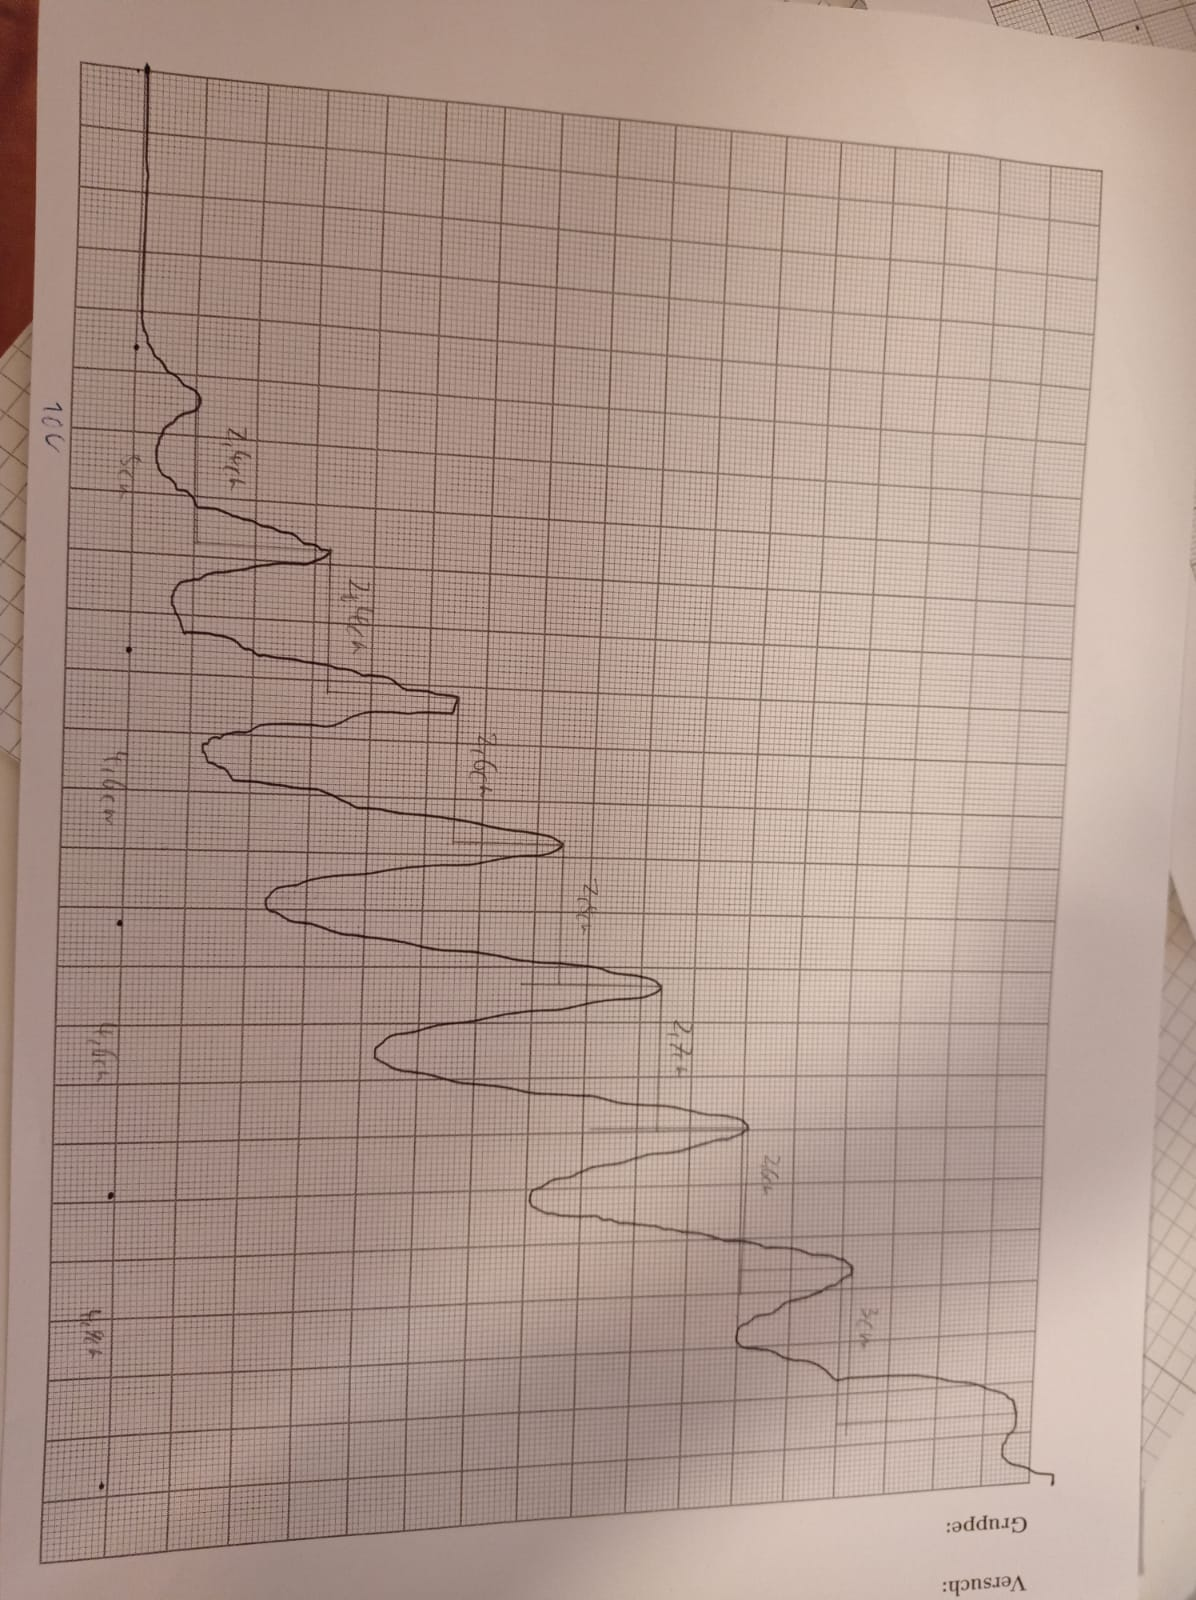
\includegraphics[width=0.7\textwidth]{latex/images/hertz.jpeg}
  \caption{Die vom x-y-Schreiber erstellte Franck-Hertz-Kurve.}
  \label{img:mess2}
\end{figure}

    \begin{figure}[h]
        \centering
        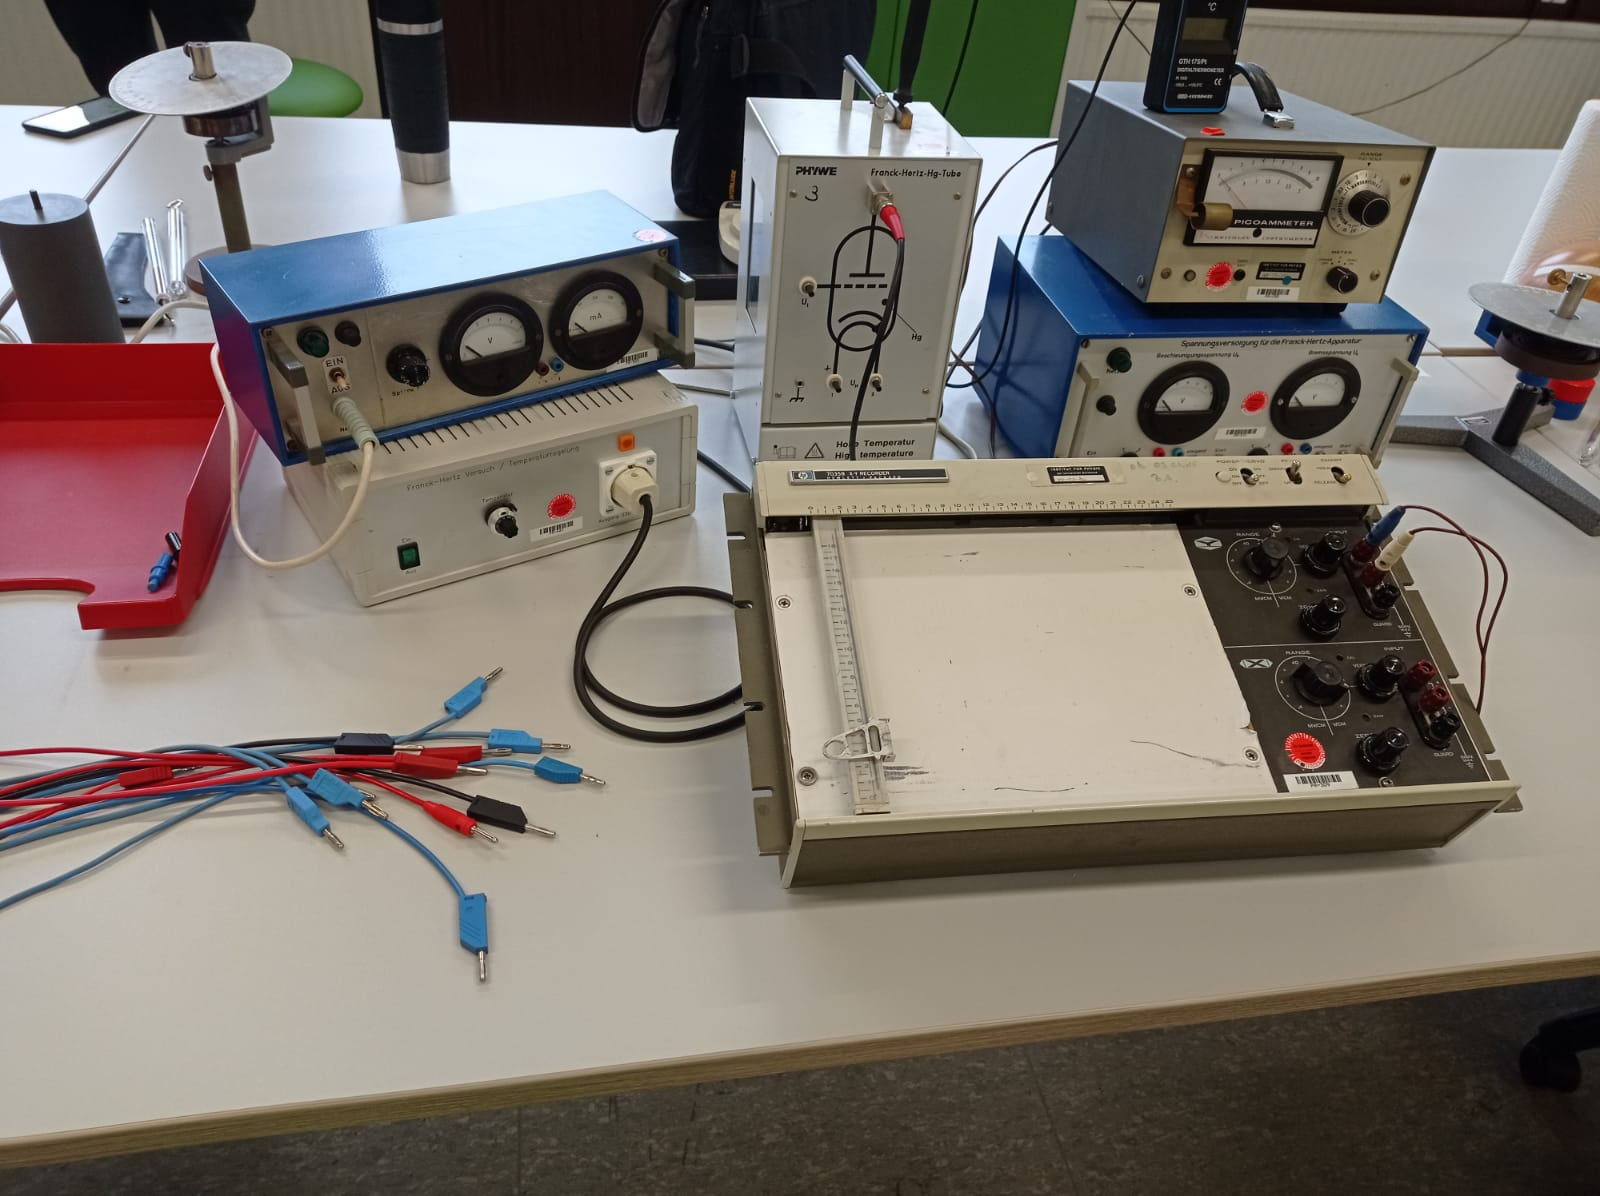
\includegraphics[width=0.7\textwidth]{latex/images/aufbau.jpeg}
        \caption{Der Versuchsaufbau mit x-y-Schreiber.}
    \end{figure}


